\documentclass[12pt,a4paper]{article}
\usepackage[UTF8]{ctex}
\usepackage{amsmath,amscd,amsbsy,amssymb,latexsym,url,bm,amsthm}
\usepackage{epsfig,graphicx,subfigure}
\usepackage{enumitem,balance}
\usepackage{wrapfig}
\usepackage{mathrsfs,euscript}
\usepackage[usenames]{xcolor}
\usepackage{hyperref}
\usepackage[vlined,ruled,linesnumbered]{algorithm2e}
\usepackage{float}
\usepackage{booktabs}
\usepackage{listings}
\usepackage{color}
\usepackage{caption}

\definecolor{mygreen}{rgb}{0,0.6,0}
\definecolor{mygray}{rgb}{0.5,0.5,0.5}
\definecolor{mymauve}{rgb}{0.58,0,0.82}
\lstset{
 backgroundcolor=\color{white}, 
 basicstyle = \footnotesize,       
 breakatwhitespace = false,        
 breaklines = true,                 
 captionpos = b,                    
 commentstyle = \color{mygreen}\bfseries,
 extendedchars = false,             
 frame =shadowbox, 
 framerule=0.5pt,
 keepspaces=true,
 keywordstyle=\color{blue}\bfseries, % keyword style
 language = Verilog,                     % the language of code
 otherkeywords={string}, 
 numbers=left, 
 numbersep=5pt,
 numberstyle=\tiny\color{mygray},
 rulecolor=\color{black},         
 showspaces=false,  
 showstringspaces=false, 
 showtabs=false,    
 stepnumber=1,         
 stringstyle=\color{mymauve},        % string literal style
 tabsize=4,          
 title=\lstname                      
}

\usepackage{fontspec}
\hypersetup{colorlinks=true,linkcolor=black}

\newtheorem{theorem}{Theorem}
\newtheorem{lemma}[theorem]{Lemma}
\newtheorem{proposition}[theorem]{Proposition}
\newtheorem{corollary}[theorem]{Corollary}
\newtheorem{exercise}{Exercise}
\newtheorem*{solution}{Solution}
\newtheorem{definition}{Definition}
\theoremstyle{definition}

\renewcommand{\thefootnote}{\fnsymbol{footnote}}

\newcommand{\postscript}[2]
 {\setlength{\epsfxsize}{#2\hsize}
  \centerline{\epsfbox{#1}}}

\renewcommand{\baselinestretch}{1.0}

\setlength{\oddsidemargin}{-0.365in}
\setlength{\evensidemargin}{-0.365in}
\setlength{\topmargin}{-0.3in}
\setlength{\headheight}{0in}
\setlength{\headsep}{0in}
\setlength{\textheight}{10.1in}
\setlength{\textwidth}{7in}
\makeatletter \renewenvironment{proof}[1][Proof] {\par\pushQED{\qed}\normalfont\topsep6\p@\@plus6\p@\relax\trivlist\item[\hskip\labelsep\bfseries#1\@addpunct{.}]\ignorespaces}{\popQED\endtrivlist\@endpefalse} \makeatother
\makeatletter
\renewenvironment{solution}[1][Solution] {\par\pushQED{\qed}\normalfont\topsep6\p@\@plus6\p@\relax\trivlist\item[\hskip\labelsep\bfseries#1\@addpunct{.}]\ignorespaces}{\popQED\endtrivlist\@endpefalse} \makeatother

% caption
\counterwithin*{figure}{section}
\counterwithin*{figure}{subsection}
\counterwithin*{figure}{subsubsection}
\renewcommand{\thefigure}{%
  \ifnum\value{subsection}=0
    \thesection.\arabic{figure}%
  \else
    \ifnum\value{subsubsection}=0
      \thesubsection.\arabic{figure}%
    \else
      \thesubsubsection.\arabic{figure}%
    \fi
  \fi
}

\counterwithin*{table}{section}
\counterwithin*{table}{subsection}
\counterwithin*{table}{subsubsection}
\renewcommand{\thetable}{%
  \ifnum\value{subsection}=0
    \thesection.\arabic{table}%
  \else
    \ifnum\value{subsubsection}=0
      \thesubsection.\arabic{table}%
    \else
      \thesubsubsection.\arabic{table}%
    \fi
  \fi
}

\begin{document}
\noindent
\captionsetup[figure]{labelfont={bf},name={Fig.}}
\captionsetup[table]{labelfont={bf},name={Tab.}}
%========================================================================

\noindent\framebox[\linewidth]{\shortstack[c]{
\Large{\textbf{DCP3362 Computer Organization Lab 2}}\vspace{1mm}\\
\footnotesize{\color{blue}$*$ Name: 石育瑋  \quad ID: A073708 \quad Email: stoneonetwo1203@gmail.com}}}

%\begin{center}
%\Large{\textbf{Computer Organization Lab 1}}\vspace{1mm}\\
%\footnotesize{\color{blue}$*$ Name: 石育瑋  \quad ID: A073708 \quad Email: yuwei.shih.tw@gmail.com}
%\end{center}

\section{Architecture diagrams}

\begin{figure}[H]
\centering
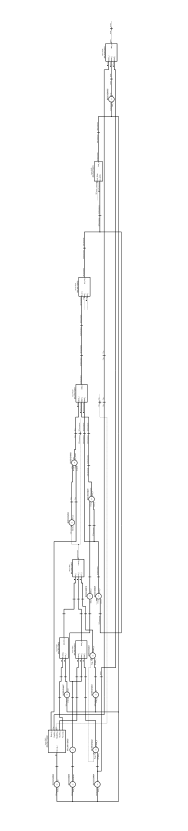
\includegraphics[height=19cm]{fig/dataflow.png}
\caption{Data flow of CPU}
\label{fig:cpu}
\end{figure}

\begin{figure}[H]
\centering
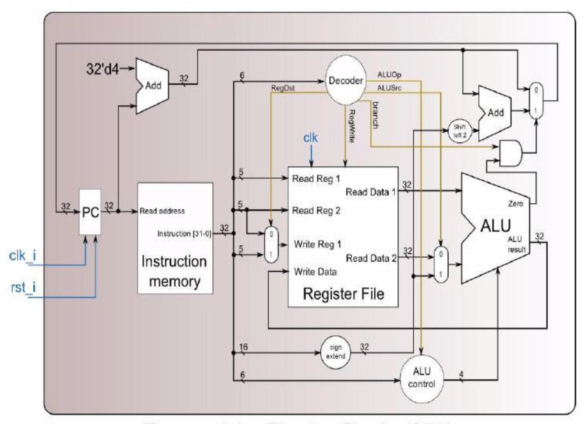
\includegraphics[height=10cm]{fig/cpu.png}
\caption{Architecture}
\label{fig:archi}
\end{figure}


\section{Hardware module analysis}

\begin{figure}[H]
\centering
\begin{lstlisting}[caption={}]
module alu_top(
               src1,       //1 bit source 1 (input)
               src2,       //1 bit source 2 (input)
               less,       //1 bit less     (input)
               A_invert,   //1 bit A_invert (input)
               B_invert,   //1 bit B_invert (input)
               cin,        //1 bit carry in (input)
               operation,  //operation      (input)
               result,     //1 bit result   (output)
               cout,       //1 bit carry out(output)
               );
\end{lstlisting}
\caption{alu$\_$top module}
\label{fig:alu_top_}
\end{figure}


在alu$\_$top的設計中:
\begin{enumerate}
\item 2個2-1 MUX 控制信號:
\begin{itemize}
\item (input) A$\_$invert
\item (input) B$\_$invert
\end{itemize}
當A$\_$invert或B$\_$invert為1時,對src1或src2取NOT值輸出;而當A$\_$invert或B$\_$invert為0時,則輸出src1或src2。

\item 1個4-1 MUX 控制信號:
\begin{itemize}
\item (input) operation
\end{itemize}
當operation為00時,進行AND運算。\\
當operation為01時,進行OR運算。\\
當operation為10時,進行ADD運算。\\
當operation為11時,進行SLT運算,搭配(input) less信號。

\item 輸出運算結果
\begin{itemize}
\item (output) result
\end{itemize}

\item 輸出進位
\begin{itemize}
\item (output) cout
\end{itemize}
\end{enumerate}

\begin{figure}[H]
\centering
\begin{lstlisting}[caption={}]
module alu(
           clk,           // system clock              (input)
           rst_n,         // negative reset            (input)
           src1,          // 32 bits source 1          (input)
           src2,          // 32 bits source 2          (input)
           ALU_control,   // 4 bits ALU control input  (input)
			  //bonus_control, // 3 bits bonus control input(input) 
           result,        // 32 bits result            (output)
           zero,          // 1 bit when the output is 0, zero must be set (output)
           cout,          // 1 bit carry out           (output)
           overflow       // 1 bit overflow            (output)
           );
\end{lstlisting}
\caption{alu module}
\label{fig:alu_}
\end{figure}

在alu的設計中:
\begin{enumerate}
\item 2個ALU控制信號:
\begin{itemize}
\item (input) clk
\item (input) rst$\_$n
\end{itemize}
當clk上沿時,才對運算結果等進行更新。\\
當rst$\_$n為1時,ALU才會運作。

\item 2個輸入srouce:
\begin{itemize}
\item (input) src1
\item (input) src2
\end{itemize}

\item ALU控制信號
\begin{itemize}
\item (input) ALU$\_$control
\end{itemize}
控制關係在表\ref{tab:support}中。

\item 4個輸出結果
\begin{itemize}
\item (output) result
\item (output) zero
\item (output) cout
\item (output) overflow
\end{itemize}
\end{enumerate}

在alu中呼叫了32個圖\ref{fig:alu_top_} alu$\_$top,其中 alu$\_$top 負責AND、OR、NOT、ADD的運算,圖\ref{fig:alu_} alu則是將所有的控制值(ex:運算的controll、invert等)傳進alu$\_$top以及對最後輸出的結果進行處理。

\section{Finished part}

實驗透過助教提供的Test Bench與ModelSim進行模擬測試,表\ref{tab:data}為輸入的測試數據表格,分別對6種不同的運算測驗,模擬出來得到的結果在表\ref{tab:result}中,圖\ref{fig:result}可以看到最終結果正確無偏差。
\begin{table}[H]
\centering
\caption
{實驗數據}
\label{tab:data}
\begin{tabular}{llll} \toprule
operation & ALU code & src1 & src2 \\
\midrule
AND & 0000 & ffff0000 & 0000ffff
\\
OR & 0001 & 3113c398 & 088e4954
\\
ADD & 0010 & ffffffff & 00000001
\\
SUB & 0110 & 7eda5023 & 2ec36ae5
\\
SLT & 0111 & ffffffff & 00000001
\\
NOR & 1100 & 00000000 & 00000000
\\ \bottomrule
\end{tabular}
\end{table}

\begin{table}[H]
\centering
\caption
{實驗結果}
\label{tab:result}
\begin{tabular}{ll} \toprule
result & zcv \\
\midrule
00000000 & 100
\\
399fcbdc & 000
\\
00000000 & 110
\\
5016e53e & 010
\\
00000001 & 000
\\
ffffffff & 000
\\ \bottomrule
\end{tabular}
\end{table}

\begin{figure}[H]
\centering
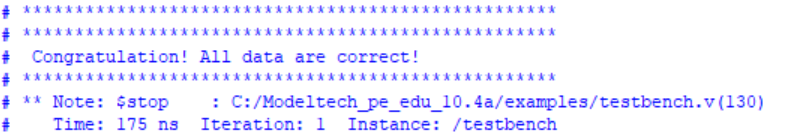
\includegraphics[width=16cm]{fig/result.png}
\caption{testbench測試結果}
\label{fig:result}
\end{figure}

\section{Problems you met and solutions}

在寫LAB時,主要有遇到以下2個問題:
\begin{enumerate}
\item 分不清楚verilog裡"A $<=$ B;"與"assign A $=$ B;"之間的差異,導致在寫lab時不知什麼情況該用哪一種。
\begin{solution}
\item
\begin{enumerate}
\item assign a = b (Blocking assignment) : 執行順序不一定,
\item a <= b (Nonblocking assignment) : 所有可同時值行的東西都要執行完一次後,才會前進到下一個時間點。
\end{enumerate}
\end{solution}

\item 在連接alu$\_$top時,不知道如何生成32個alu$\_$top modules。
\begin{solution}
\item 先創建初始第一個alu$\_$top alu$\_$0,再利用for循環創建剩餘的31個alu$\_$top,最後將less wire連接。

\begin{figure}[H]
\centering
\begin{lstlisting}[caption={}]
// construct ALU from alu_top
alu_top  alu_0(
    .src1(src1[0]),
    .src2(src2[0]),
    .less(!carry_wire[31]),
    .A_invert(ALU_control[3]),
    .B_invert(ALU_control[2]),
    .cin(1'b0),
    .operation(ALU_control[1:0]),
    .result(result_wire[0]),
    .cout(carry_wire[0])
);
for(i=1; i<32; i=i+1) begin: generate_alu_top
    alu_top  alu_k(
        .src1 (src1[i]),
        .src2 (src2[i]),
        .less (1'b0),
        .A_invert (ALU_control[3]),
        .B_invert (ALU_control[2]),
        .cin (carry_wire[i-1]),
        .operation (ALU_control[1:0]),
        .result (result_wire[i]),
        .cout (carry_wire[i])
    );
end
\end{lstlisting}
\caption{Construct ALU from alu$\_$top}
\label{fig:construct}
\end{figure}
\end{solution}

\end{enumerate}

\section{Summary}


這個Lab是我第一次接觸Verilog,學到很多東西,對計算機組織中ALU的架構也更加理解,最終實現表\ref{tab:support}中的6種指令。

\begin{table}[H]
\centering
\caption
{Supported Instructions}
\label{tab:support}
\begin{tabular}{llc} \toprule
ALU Action & Name & ALU Control Input \\
\midrule
And & And & 0000
\\
Or & Or & 0001
\\
Add & Addition & 0010
\\
Sub & Subtraction & 0110
\\
Nor & Nor & 1100
\\
Slt & Set less than & 0111
\\ \bottomrule
\end{tabular}
\end{table}




%========================================================================
\end{document}
